%\documentclass[wsdraft]{ws-procs11x85}

\documentclass{ws-procs11x85}
\usepackage{ws-procs-thm}           % comment this line when `amsthm / theorem / ntheorem` package is used

\begin{document}

\title{Improving QSAR Modeling for Predictive Toxicology using Publicly Aggregated Semantic Graph Data and Graph Neural Networks}

\author{Joseph~D.~Romano$^*$, Yun~Hao$^*$, and Jason~H.~Moore$^\dag$}

\address{Institute for Biomedical Informatics, University of Pennsylvania,\\
Philadelphia, Pennsylvania 19104, United States\\
$^\dag$E-mail: jhmoore@upenn.edu\\
$^*$These authors contributed equally.}

\begin{abstract}
Quantitative Structure-Activity Relationship (QSAR) modeling is the most common computational technique for predicting toxicity for specific chemicals, but a lack of methodological innovations have led to underwhelming performance of QSAR in modern applications.
We show that contemporary QSAR modeling for predictive toxicology can be substantially improved by incorporating semantic graph data aggregated from open-access public databases, and analyzing those data in the context of graph neural networks (GNNs).
Furthermore, we introspect the GNNs to demonstrate how they can lead to more interpretable applications of QSAR, and use ablation analysis to explore the contribution of different data elements to the final models' performance.
\end{abstract}

\keywords{Toxicology; Graph neural networks; Data aggregation; QSAR; Artificial intelligence.}

\section{Introduction}\label{aba:sec1}
Testing.

\section{Methods}

\subsection{Aggregating publicly accessible multimodal graph data}
The graph data used in this study come from a new data resource for computational toxicology, named ComptoxAI.
ComptoxAI includes a large graph database containing many entity and relationship types that pertain to translational mechanisms of toxicity, all of which are sourced from third-party public databases (including PubChem, Drugbank, the US EPA's Computational Toxicology Dashboard, NCBI Gene, and many others).
We extracted the subgraph from ComptoxAI's graph database defined as all nodes representing chemicals, genes, and toxicological assays, as well as the complete set of edges linking nodes of those types.
A metagraph describing the node and edge types in the subgraph is shown in [FIGURE XXX].

Every prediction task in this study involves QSAR modeling between chemicals of toxicological interest and toxicology-related activity assays derived from the US EPA's Tox21 dataset.
Each chemical and assay is represented as a node within the larger graph database, and all chemical--assay pairs are either linked by an edge (\textit{chemicalHasActiveAssay} or \textit{chemicalHasInactiveAssay}) or not linked by an edge (i.e., no data has been collected on the chemical with respect to the assay in question). 

\subsection{Obtaining toxicology assay data}
We used the Tox21 dataset---which is a freely available resource produced collaboratively by the US National Institutes of Health, the US Food and Drug Administration, and the US Environmental Protection Agency---to obtain a set of candidate assays for classification and establish `ground truth' relationships between specific chemicals and those assays.

\subsection{Heterogeneous graph neural network}
We constructed a heterogeneous graph convolutional neural network (GCNN) architecture for the graph ML experiments.
Since our approach uses multiple entity types (e.g., chemicals, genes, assays) in the same graph---each with possibly different sets of node features, and linked by multiple semantically distinct edge types---the architecture extends the common GCNN model to learn separate message passing functions for each edge type.
Briefly, each layer of the network aggregates signals from adjacent nodes in the graph, such that a greater number of layers results in signals being aggregated from an increasingly wider radius around each node.
The output of the network can be thought of as encoded representations of nodes that incorporate information from other nodes in their local neighborhood.
Additionally, GCNNs can be thought of as a generalization of convolutional neural networks (CNNs) used in computer vision---instead of the convolutional operator aggregating signals from nearby pixels in an image, it aggregates features from adjacent nodes in the graph.

In a heterogeneous graph, different node types represent different types of entities, each represented within a semantically distinct feature space.
Therefore, the process of aggregating information from adjacent nodes must take those nodes' types into account.
Additionally, different edge types (e.g., `chemicalUpregulatesGene' and `chemicalDownregulatesGene') convey their own semantically distinct meanings, which can substantially effect the flow of information through the network.
To handle these two challenges, we learn separate aggregation functions for each edge type in the graph, following the example proposed by Schlichtkrull \textit{et al} in R-GCNs (Relational Graph Convolutional Networks)~\cite{schlichtkrull2018modeling}.
Within the R-GCN paradigm, the aggregation process can be split into 3 sequential steps: (1.)~collecting signals from adjacent nodes using an appropriate edge type-specific message function $\phi$, (2.)~combining each of those incoming signals (across all edge types) via a reduce function $\rho$, and (3.)~finally updating the target node $v$ by applying an update function $\psi$.
Training the network is roughly equivalent to finding an appropriate parameterization of $\phi$ for each edge type.

A formal description of the GNN is given in \textbf{Appendix~\ref{GCNN}}.

% We use a message passing strategy similar to GraphSAGE~\cite{hamilton2017inductive}, where signals propagated from adjacent nodes are aggregated using their arithmetic mean:
% \begin{equation}
% \mathbf{h}_v^k \gets \sigma\left(\mathbf{W} \cdot \textsc{Mean}(\{\mathbf{h}_v^{k-1}\}\cup \{ \mathbf{h}_u^{k-1},\forall u \in \mathcal{N}(v) \})\right)
% \end{equation}
% where $\mathbf{h}_v^{k}$ is an encoded representation of the input vector $\mathbf{x}$ of node $v$ at layer $k$ of the network, $\mathbf{W}$ is a weight matrix, and $\mathcal{N}(v)$ is the neighborhood of all nodes adjacent to $v$.
% Each layer in the network `pulls' information from an increasingly wider radius around each node $v$.
% $\sigma$ is an activation applied to the output of each layer, which we define as the leaky ReLU function:
% \begin{equation}
% \sigma(x) =
% \begin{cases}
%    x & \quad \text{if } x > 0,\\
%    0.01x & \quad \text{otherwise}
% \end{cases}
% \end{equation}

\subsubsection{Node classification model}
Our node classification task consists of labeling chemicals according to whether they do (1) or do not (0) activate a specific Tox21 assay.
The procedure we use for generating these labels is as follows:
\begin{enumerate}
   \item For each $c \in \mathcal{C}$ is adjacent to the assay of interest $a \in \mathcal{A}$, generate labels according to the following scheme:
   \begin{enumerate}
      \item 1 if there exists an edge $(c, r, a)$ such that the edge type of $r$ is \texttt{chemicalHasActiveAssay}.
      \item 0 if there exists an edge $(c, r, a)$ such that the edge type of $r$ is \texttt{chemicalHasInactiveAssay}.
      \item If both of the two preceding conditions are false, no label is generated.
   \end{enumerate}
   \item Delete $a$ (and all edges incident to $a$) from the graph.
\end{enumerate}
The resulting graph $\mathcal{G}_a^\star$ is then used in a standard supervised learning task where the goal is to predict the labels on nodes corresponding to chemicals, which represent whether the assay is or is not activated in response to perturbation by that chemical.
We use an 80\%/20\% train/test split on the labeled chemicals, optimize the GCNN's parameters using the Adam algorithm (a computationally efficient variant of stochastic gradient descent suitable for sparse gradients)~\cite{kingma2014adam}, and compute the error between predicted and true labels via cross entropy loss.

To assess the contribution of the MACCS molecular descriptors when added to the GNN, we trained the node classification model both in the presence and in the absence of MACCS bitstrings applied as node features to each chemical.
Intuitively, the model trained without MACCS node features performs inference using only the graph's topological structure---including gene interactions and activity annotations to the other Tox21 assays---while the one with MACCS node features additionally has access to the same chemical structure information used in the non-graph (baseline) QSAR models.

Specific details for the node classification task are given in \textbf{Appendix~\ref{NC}}.

\subsection{Baseline QSAR classifiers}

\section{Results}
\subsection{GCNN performance on node classification and comparison to baseline QSAR models}

\begin{figure}
   \includegraphics[width=\textwidth]{figures/figure2.pdf}
\end{figure}

\begin{figure}
   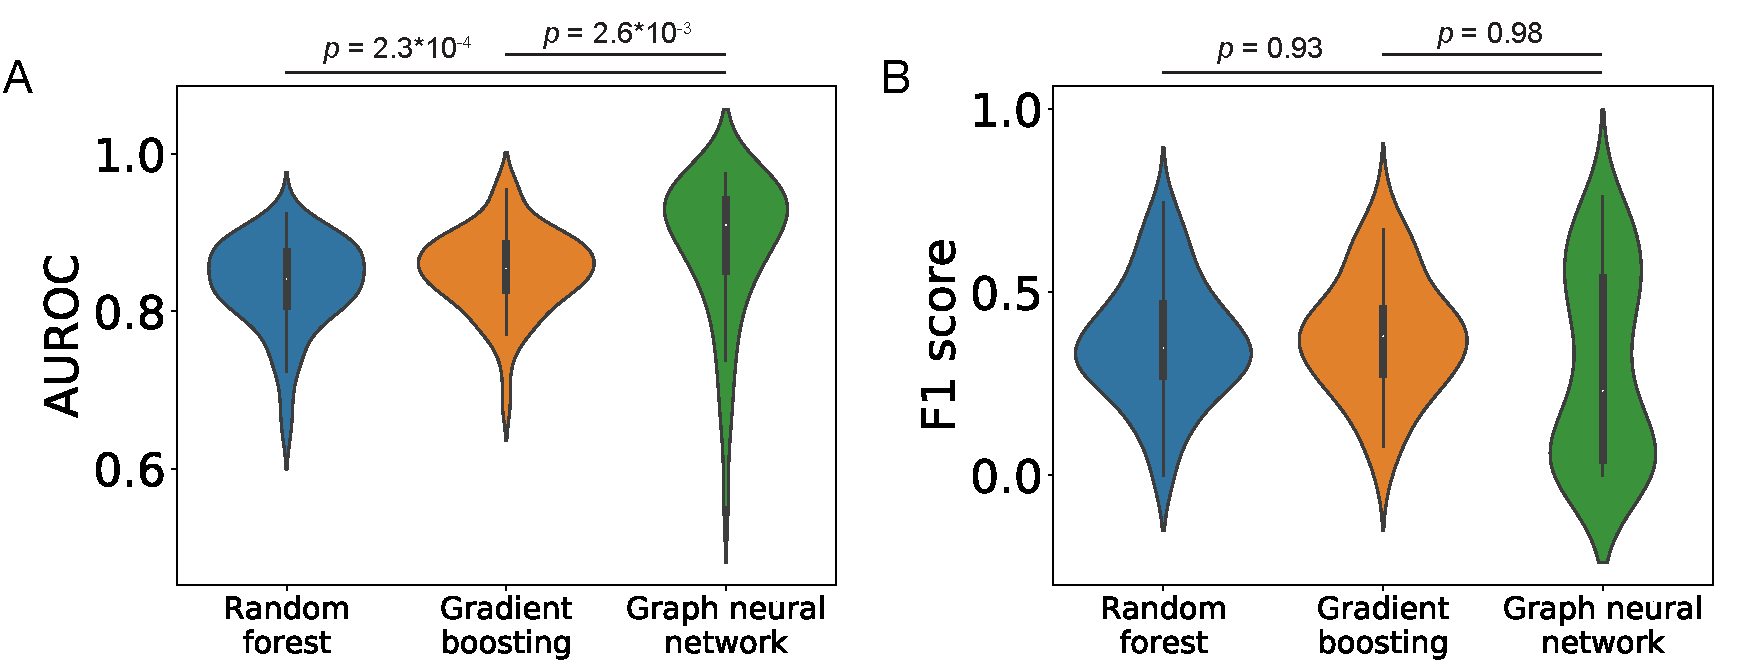
\includegraphics[width=\textwidth]{figures/figure3.pdf}
\end{figure}

\subsection{Ablation analysis of graph components' influence on the trained predictive model}

\subsection{Interpretability of trained GCNNs via assay embeddings}

\section{Discussion}

\section{Conclusions}

\section{Code availability}
All source code pertaining to this study is available on GitHub at \url{https://github.com/EpistasisLab/qsar-gnn}.
A frozen copy of the code at the time of writing is available at [XXX; Zenodo].

\section{Supplemental Materials}
Supplemental tables and figures are available on FigShare at [XXX].

\section*{Acknowledgements}
This work was made possible with support from US National Institutes of Health grants \texttt{R01-LM010098}, \texttt{R01-LM012601}, \texttt{R01-AI116794}, \texttt{UL1-TR001878}, \texttt{UC4-DK112217} (PI: Jason~Moore), \texttt{T32-ES019851}, and \texttt{P30-ES013508} (PI: Trevor~Penning).

\bibliographystyle{ws-procs11x85}
\bibliography{psb-gnn}

\appendix{Graph convolutional network architecture}\label{GCNN}
Some stuff here.

\appendix{Node classification model}\label{NC}
Some more stuff.

\end{document} 

%%% \renewcommand\bibname{References\\ {\normalfont\it References can be typed in your preferred bibliography style.}}